\chapter{Praktická část}

Postup řešení a dosažené výsledky dle povahy projektu.
\\\\
\noindent
\textbf{Případová studie}:
\begin{itemize}
    \item určení zkoumané oblasti,
    \item zvolená metodika řešení,
    \item průzkum a testování,
    \item nálezy a komentáře.
\end{itemize}
\textbf{Vývoj nástroje}:
\begin{itemize}
    \item vysokoúrovňový návrh,
    \item použité technologie,
    \item vlastní implementace,
    \item testování a ukázky.
\end{itemize}

\begin{figure}[ht!]
    \centering
    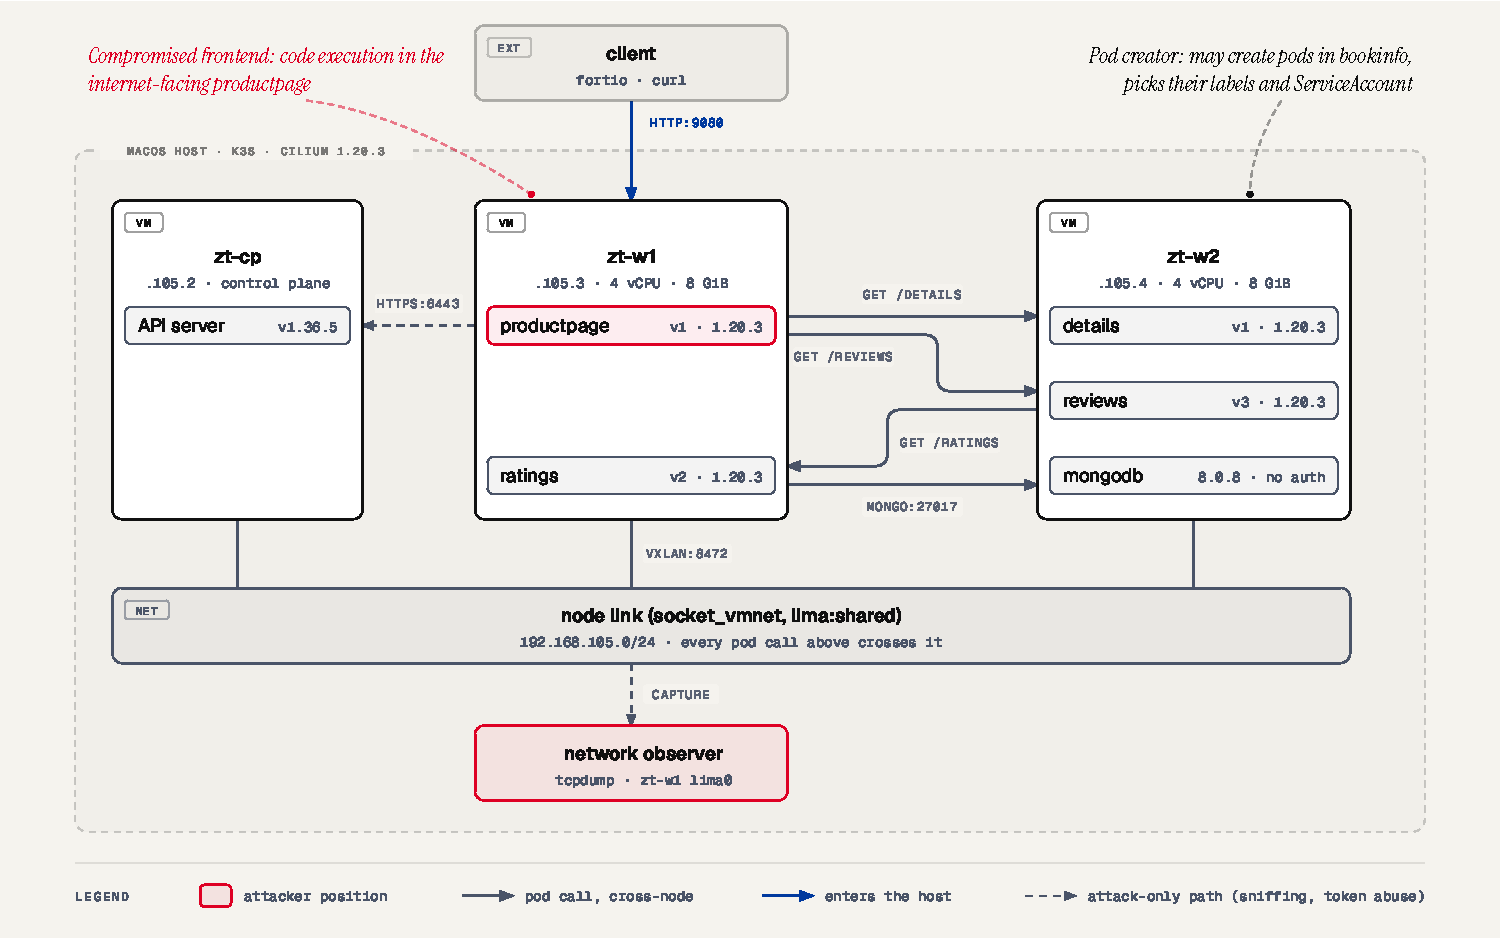
\includegraphics[width=\textwidth]{../figures/testbed.pdf}
    \caption{Testbed: Bookinfo on three VMs; every call crosses nodes, attacker positions AT1 to AT3.}
    \label{fig:testbed}
\end{figure}

\begin{figure}[ht!]
    \centering
    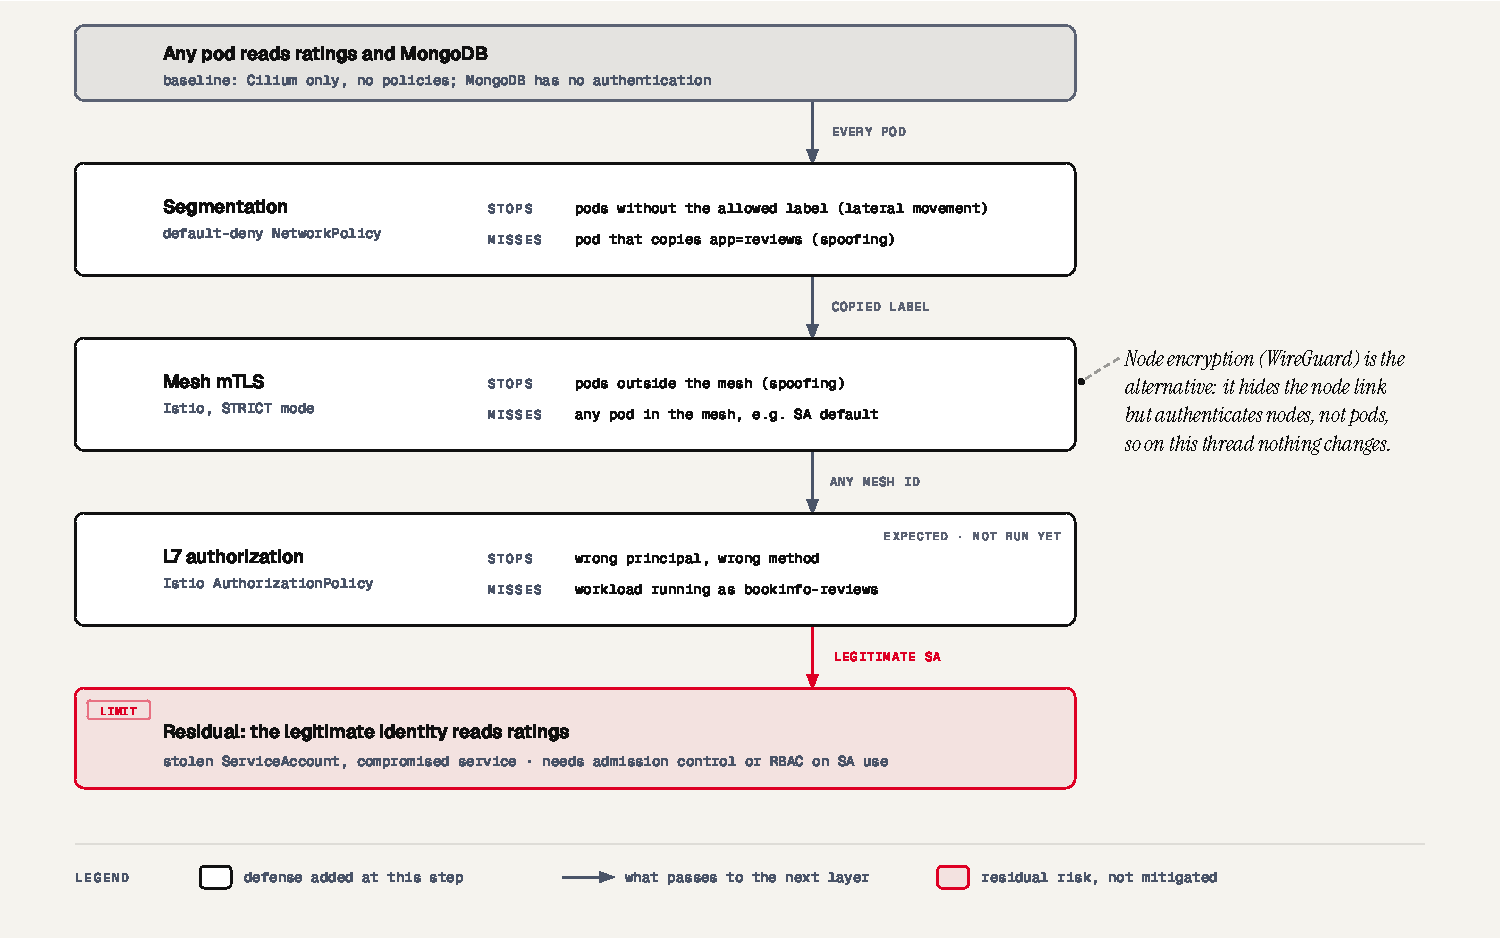
\includegraphics[width=\textwidth]{../figures/scenario-layers.pdf}
    \caption{What each scenario stops on the path to the ratings data, and the residual risk.}
    \label{fig:scenario-layers}
\end{figure}
